% The Widening Edge: Remoteness, Acceleration and the Connectivity Tax
% Build with `make pdf` from the repository root (LuaLaTeX + biber).
\documentclass[11pt,letterpaper,oneside]{article}

% ------------------------------------------------------------------ palette
\usepackage{xcolor}
% Brand palette. Teal and ember differ strongly in lightness as well as hue,
% so they stay distinguishable in greyscale and for common colour-vision
% deficiencies; sand is reserved for counterpoint material.
\definecolor{teal}{HTML}{0F5E66}     % primary
\definecolor{ember}{HTML}{D9622B}    % accent
\definecolor{sand}{HTML}{E9C46A}     % counterpoints
\definecolor{mist}{HTML}{EEF5F5}     % backgrounds
\definecolor{ink}{HTML}{1E2A2C}      % body text (soft black)
\definecolor{slate}{HTML}{6B7B7D}    % secondary text, axes
\definecolor{haze}{HTML}{C9D6D7}     % gridlines, non-highlighted points
\colorlet{tealLight}{teal!45!white}
\colorlet{sandDeep}{sand!70!black}

% ------------------------------------------------------------------ page
\usepackage[letterpaper,top=1in,bottom=1in,left=1.1in,right=1.1in,
            headheight=14pt,headsep=22pt,footskip=30pt]{geometry}

% ------------------------------------------------------------------ fonts
% EB Garamond for text with its matching Garamond-Math; Source Sans for
% headings furniture, figures and tables.
\usepackage{fontspec}
\usepackage{unicode-math}
\setmainfont{EBGaramond}[
  Extension=.otf, UprightFont=*-Regular, ItalicFont=*-Italic,
  BoldFont=*-SemiBold, BoldItalicFont=*-SemiBoldItalic,
  Numbers={OldStyle,Proportional}, Ligatures=TeX]
\newfontfamily\liningfigures{EBGaramond}[
  Extension=.otf, UprightFont=*-Regular, ItalicFont=*-Italic,
  BoldFont=*-SemiBold, Numbers={Lining,Monospaced}]
\setsansfont{SourceSansPro}[
  Extension=.otf, UprightFont=*-Regular, ItalicFont=*-RegularIt,
  BoldFont=*-Semibold, BoldItalicFont=*-SemiboldIt,
  Scale=MatchLowercase]
\newfontfamily\sanslight{SourceSansPro}[
  Extension=.otf, UprightFont=*-Light, ItalicFont=*-LightIt,
  BoldFont=*-Semibold, Scale=MatchLowercase]
\setmathfont{Garamond-Math.otf}[StylisticSet={7,9}]

\usepackage[babel=true]{microtype}
\usepackage[english]{babel}
\usepackage{csquotes}
\linespread{1.12}
\setlength{\parindent}{1.2em}
\setlength{\parskip}{0pt}
\color{ink}

% ------------------------------------------------------------------ packages
\usepackage{graphicx}
\usepackage{booktabs}
\usepackage{tabularx}
\usepackage{array}
\usepackage{multirow}
\usepackage{enumitem}
\setlist{itemsep=2pt,topsep=4pt,leftmargin=1.4em}
\usepackage{siunitx}
\sisetup{group-minimum-digits=4,group-separator={,}}
\usepackage{xcolor}
\usepackage{caption}
\usepackage{subcaption}
\usepackage{float}
\usepackage{etoolbox}
\usepackage{xparse}

% ------------------------------------------------------------------ headings
\usepackage[explicit]{titlesec}
\titleformat{\section}
  {\normalfont\Large\color{teal}}
  {\makebox[2.2em][l]{\sffamily\bfseries\large\color{ember}\thesection}}
  {0pt}{\scshape\MakeLowercase{#1}}
\titleformat{\subsection}
  {\normalfont\large\itshape\color{teal}}
  {\thesubsection}{0.8em}{#1}
\titleformat{\paragraph}[runin]
  {\normalfont\sffamily\bfseries\small\color{teal}}{}{0pt}{#1}[\quad]
\titlespacing*{\section}{0pt}{2.2\baselineskip}{1.0\baselineskip}
\titlespacing*{\subsection}{0pt}{1.4\baselineskip}{0.5\baselineskip}
\titlespacing*{\paragraph}{0pt}{0.8\baselineskip}{0pt}

% ------------------------------------------------------------------ header
\usepackage{fancyhdr}
\pagestyle{fancy}
\fancyhf{}
\fancyhead[L]{\sffamily\footnotesize\color{slate}\textsc{The Widening Edge}}
\fancyhead[R]{\sffamily\footnotesize\color{slate}Working Paper}
\fancyfoot[C]{\sffamily\footnotesize\color{slate}\thepage}
\renewcommand{\headrulewidth}{0.4pt}
\renewcommand{\headrule}{\hbox to\headwidth{\color{haze}\leaders\hrule height \headrulewidth\hfill}}
\fancypagestyle{plain}{\fancyhf{}\renewcommand{\headrulewidth}{0pt}
  \fancyfoot[C]{\sffamily\footnotesize\color{slate}\thepage}}

% ------------------------------------------------------------------ captions
% Captions lead with the takeaway (bold), then the detail and source.
\DeclareCaptionFont{capsans}{\sffamily\small}
\DeclareCaptionLabelFormat{brand}{\textcolor{ember}{\bfseries #1 #2}}
\captionsetup{font=capsans,labelformat=brand,labelsep=quad,
  justification=raggedright,singlelinecheck=false,skip=6pt}
\captionsetup[table]{position=top}
\newcommand{\takeaway}[1]{\textbf{\color{teal}#1}\enspace}
\newcommand{\source}[1]{\par\smallskip{\footnotesize\color{slate}\textit{Source:} #1}}

% ------------------------------------------------------------------ links
\usepackage[hidelinks=false,colorlinks=true,linkcolor=teal,citecolor=teal,
  urlcolor=ember,filecolor=ember,pdfpagelabels,bookmarksnumbered]{hyperref}
\usepackage[nameinlink,noabbrev]{cleveref}
\crefname{figure}{Figure}{Figures}
\crefname{table}{Table}{Tables}
\crefname{section}{Section}{Sections}

% ------------------------------------------------------------------ bibliography
\usepackage[backend=biber,style=authoryear-comp,maxcitenames=2,
  uniquelist=false,uniquename=false,dashed=false,giveninits=true,
  doi=true,url=false,isbn=false,eprint=false]{biblatex}
\DeclareFieldFormat{doi}{\mkbibacro{DOI}\addcolon\space\href{https://doi.org/#1}{\nolinkurl{#1}}}
\renewcommand*{\bibfont}{\small}
\setlength{\bibitemsep}{3pt}

% ------------------------------------------------------------------ data macros
% \placeholder{text} marks content that is not yet backed by data. It renders
% in ember on a sand background, writes a line to the log, and is a hard
% error in `make final` (which defines \finalbuild).
\NewDocumentCommand{\placeholder}{m}{%
  \ifdefined\finalbuild
    \PackageError{widening-edge}{Placeholder remains: #1}{Replace with data.}%
  \fi
  \typeout{PLACEHOLDER: #1}%
  {\sffamily\small\colorbox{sand!40}{\color{ember}[\,#1\,]}}}

% ------------------------------------------------------------------ components
\usepackage[most]{tcolorbox}

% Abstract: mist panel with a teal top rule.
\newtcolorbox{abstractbox}{enhanced,breakable,colback=mist,colframe=mist,
  boxrule=0pt,arc=0pt,left=14pt,right=14pt,top=10pt,bottom=12pt,
  borderline north={2pt}{0pt}{teal},
  fontupper=\small\linespread{1.15}\selectfont,
  title={\sffamily\bfseries\footnotesize\color{teal}\MakeUppercase{Abstract}},
  coltitle=teal,colbacktitle=mist,attach title to upper={\par\smallskip}}

% Pull quote: large italic, teal left rule.
\newtcolorbox{pullquote}{enhanced,breakable=false,colback=white,colframe=white,
  boxrule=0pt,arc=0pt,left=14pt,right=10pt,top=4pt,bottom=4pt,
  borderline west={3pt}{0pt}{teal},before skip=14pt,after skip=14pt,
  fontupper=\Large\itshape\color{teal}\linespread{1.05}\selectfont}

% Key idea: ember accent.
\newtcolorbox{keyidea}[1][Key Idea]{enhanced,breakable,colback=ember!6,
  colframe=ember!6,boxrule=0pt,arc=1pt,left=12pt,right=12pt,top=8pt,bottom=8pt,
  borderline west={3pt}{0pt}{ember},before skip=12pt,after skip=12pt,
  fontupper=\small,
  title={\sffamily\bfseries\footnotesize\MakeUppercase{#1}},coltitle=ember,
  attach title to upper={\par\smallskip}}

% Counterpoint: sand panel for the strongest objections to the argument.
\newtcolorbox{counterpoint}[1][Counterpoint]{enhanced,breakable,colback=sand!22,
  colframe=sand!22,boxrule=0pt,arc=1pt,left=12pt,right=12pt,top=8pt,bottom=8pt,
  borderline west={3pt}{0pt}{sandDeep},before skip=12pt,after skip=12pt,
  fontupper=\small,
  title={\sffamily\bfseries\footnotesize\MakeUppercase{#1}},
  coltitle=sandDeep!80!black,attach title to upper={\par\smallskip}}

% At-a-glance claim tiles.
\newtcolorbox{claimtile}[1]{enhanced,colback=mist,colframe=mist,boxrule=0pt,
  arc=0pt,left=10pt,right=10pt,top=8pt,bottom=8pt,
  borderline north={2pt}{0pt}{teal},equal height group=claims,
  fontupper=\small\raggedright,
  title={\sffamily\bfseries\color{ember}#1},attach title to upper={\par\smallskip}}

% ------------------------------------------------------------------ plots
\usepackage{pgfplots}
\pgfplotsset{compat=1.18}
\usepgfplotslibrary{groupplots,fillbetween,colorbrewer}
\usetikzlibrary{arrows.meta,positioning,calc,decorations.markings,shapes.geometric,shadows}
\pgfplotsset{table/col sep=comma}

% Data directory (relative to paper/).
\newcommand{\datadir}{../data/processed}

% House style shared by every chart: sans labels, light grid, no top/right box.
\pgfplotsset{
  edge/.style={
    width=\linewidth, height=0.58\linewidth,
    axis lines*=left,
    axis line style={slate,line width=0.5pt},
    tick style={slate,line width=0.4pt},
    major tick length=3pt,
    tick label style={font=\sffamily\scriptsize,color=slate},
    label style={font=\sffamily\footnotesize,color=ink},
    title style={font=\sffamily\small\bfseries,color=ink},
    legend style={font=\sffamily\scriptsize,draw=none,fill=none,
                  text=ink,cells={anchor=west}},
    legend cell align=left,
    grid=major, grid style={haze,line width=0.3pt,dash pattern=on 1pt off 1.5pt},
    every axis plot/.append style={line join=round},
    scaled ticks=false,
    /pgf/number format/1000 sep={,},
    clip marker paths=true,
  },
  % series styles: distinguishable by lightness, marker and dash in greyscale
  lineTeal/.style={teal,line width=1.6pt},
  lineEmber/.style={ember,line width=1.6pt,dashed,dash pattern=on 4pt off 2pt},
  lineSlate/.style={slate,line width=1.1pt,dash pattern=on 1pt off 1.5pt},
  lineSand/.style={sandDeep,line width=1.3pt},
  bandTeal/.style={fill=teal,fill opacity=0.12,draw=none},
  bandEmber/.style={fill=ember,fill opacity=0.12,draw=none},
  % scatter layers: background (all countries), highlight (SIDS), labels
  dotsBase/.style={only marks,mark=*,mark size=1.3pt,
    mark options={fill=haze,draw=white,line width=0.2pt}},
  dotsSIDS/.style={only marks,mark=*,mark size=1.9pt,
    mark options={fill=ember,draw=white,line width=0.3pt}},
  dotsLLDC/.style={only marks,mark=square*,mark size=1.6pt,
    mark options={fill=teal,draw=white,line width=0.3pt}},
  dotsEscape/.style={only marks,mark=diamond*,mark size=2.6pt,
    mark options={fill=sand,draw=ink,line width=0.4pt}},
  pointlabel/.style={font=\sffamily\tiny,color=ink,inner sep=1pt},
  fitline/.style={ink,line width=0.8pt,dash pattern=on 3pt off 2pt,opacity=0.7},
}


\addbibresource{references.bib}

% Generated numbers: every figure quoted in the prose comes from here.
\InputIfFileExists{../generated/stats.tex}{}{%
  \PackageWarning{widening-edge}{generated/stats.tex missing: run `make data`}}

\newcommand{\papertitle}{The Widening Edge}
\newcommand{\papersubtitle}{Remoteness, Acceleration and the Connectivity Tax}
\newcommand{\paperauthor}{Oddur}

\hypersetup{
  pdftitle={\papertitle: \papersubtitle},
  pdfauthor={\paperauthor},
  pdfsubject={Economic geography of small and remote states},
  pdfkeywords={remoteness, small island developing states, connectivity,
    economic geography, technology diffusion, brain drain, climate vulnerability},
  pdfcreator={LuaLaTeX},
}

\begin{document}

% ------------------------------------------------------------------ title page
\begin{titlepage}
\thispagestyle{empty}
\newgeometry{top=1.1in,bottom=0.9in,left=1.1in,right=1.1in}
\begin{tikzpicture}[remember picture,overlay]
  \fill[teal] (current page.north west) rectangle ([yshift=-0.42in]current page.north east);
  \fill[ember] ([yshift=-0.42in]current page.north west) rectangle ([yshift=-0.47in]current page.north east);
\end{tikzpicture}

{\sffamily\footnotesize\color{slate}\MakeUppercase{Working Paper}\enspace\textbar\enspace
 \liningfigures\the\year\par}
\vspace{1.6in}

{\fontsize{46}{48}\selectfont\color{teal}\papertitle\par}
\vspace{10pt}
{\fontsize{20}{25}\selectfont\itshape\color{ink}\papersubtitle\par}
\vspace{18pt}
{\color{ember}\rule{1.4in}{2pt}\par}
\vspace{18pt}
{\large\scshape\color{ink}\paperauthor\par}

\vspace{0.8in}
\begin{minipage}{0.82\linewidth}
\begin{pullquote}
The equalisers of our age are also the multipliers of distance.
\end{pullquote}
\end{minipage}

\vfill
\begin{abstractbox}
The technologies that were supposed to abolish distance---container shipping,
fibre-optic cables, the internet, cheap flights---have made the world more
integrated and faster-moving. This paper argues that for the most remote and
smallest economies these same forces turn remoteness from a one-off cost into
a \emph{recurring tax on participation}, paid on every shipment, byte,
specialist and negotiation. Using a reproducible pipeline of public data for
\nCountriesRemote{} economies, I separate being \emph{far} (GDP-weighted
distance to world output) from being \emph{small} (population). Distance, not
size, carries the income penalty: conditional on governance, doubling
remoteness is associated with \regDoubleRemotePctAbs\% lower income per head,
while population matters little. The evidence on a \emph{widening} gap is
mixed and reported as such: access to the internet has converged sharply,
and shipping gaps with the old hubs have narrowed; but connectivity at the
edge has stagnated relative to the median country, intensive use of new
technology remains far apart, and small islands lose a majority of their
graduates. Iceland, the Faroes, Singapore and Mauritius show that the edge is
not destiny---though, notably, the richest of them are small rather than
far. Remoteness is best understood as a trajectory that policy can bend:
through pooled scale, redundancy, vulnerability-based finance and circular
talent.

\end{abstractbox}

\vspace{10pt}
{\sffamily\scriptsize\color{slate}
Every number in this paper is produced by a script from a cited public
dataset; see the Data Appendix and the repository's \texttt{data/SOURCES.md}.
Keywords: remoteness; small island developing states; connectivity;
economic geography; technology diffusion; brain drain; climate vulnerability.\par}
\restoregeometry
\end{titlepage}

% ------------------------------------------------------------------ at a glance
\clearpage
\thispagestyle{plain}
\section*{At a Glance}
\addcontentsline{toc}{section}{At a Glance}

{\large\itshape\color{teal} Remoteness is no longer a fixed cost paid once.
It is a recurring tax, and the taxes compound.\par}
\vspace{14pt}

\noindent
\begin{minipage}[t]{0.32\linewidth}
\begin{claimtile}{1\enspace Far, not small}
Distance carries the income penalty. Conditional on governance, doubling
economic remoteness goes with \regDoubleRemotePctAbs\% lower income per head;
population barely matters (\cref{sec:edge}).
\end{claimtile}
\end{minipage}\hfill
\begin{minipage}[t]{0.32\linewidth}
\begin{claimtile}{2\enspace Arrival converges, intensity doesn't}
New technologies reach the edge within about a decade, not \lagOldMedian{} years.
But broadband, bandwidth and redundancy still lag: \nSIDSOneCable{} island
states hang on one cable or none (\cref{sec:tech,sec:accel}).
\end{claimtile}
\end{minipage}\hfill
\begin{minipage}[t]{0.32\linewidth}
\begin{claimtile}{3\enspace The edge is not destiny}
Iceland, the Faroes, Singapore and Mauritius escaped through rents,
institutions and becoming hubs. But even escapees export talent: Mauritius
lost \emigMauritius\% of its graduates (\cref{sec:escape}).
\end{claimtile}
\end{minipage}

\vspace{18pt}
\noindent{\sffamily\bfseries\small\color{teal}Headline chart\enspace}{\sffamily\small\color{slate}Access versus intensity, medians per 100 people}
\par\smallskip
\begin{center}
\begin{tikzpicture}
\begin{axis}[edge, width=0.92\linewidth, height=0.42\linewidth,
    xmin=1998, xmax=2023, xtick={2000,2005,2010,2015,2020},
    x tick label style={/pgf/number format/1000 sep={}},
    ymin=0, ymax=100,
    legend style={at={(0.02,0.98)},anchor=north west}, legend columns=2]
  \addplot[lineSlate] table[x=year,y=net_hic] {\datadir/internet_groups.csv};
  \addlegendentry{Online, rich}
  \addplot[lineTeal] table[x=year,y=net_sids] {\datadir/internet_groups.csv};
  \addlegendentry{Online, islands}
  \addplot[lineSlate, dashed, line width=1.1pt] table[x=year,y=bb_hic] {\datadir/internet_groups.csv};
  \addlegendentry{Broadband, rich}
  \addplot[lineEmber] table[x=year,y=bb_sids] {\datadir/internet_groups.csv};
  \addlegendentry{Broadband, islands}
\end{axis}
\end{tikzpicture}
\end{center}
{\sffamily\footnotesize\color{slate}
Small island states have nearly caught up on being online
(\netSidsLast\% vs \netHicLast\% in \windowEnd) but not on fixed broadband
(\bbSidsLast{} vs \bbHicLast{} lines per 100). Source: World Bank WDI; see
\cref{fig:internet}.\par}

\vspace{14pt}
\begin{counterpoint}[What the data do not show]
Remote places have not, in general, become poorer: most gained in absolute
terms. Several gaps have \emph{narrowed} (internet access; shipping relative
to the old hubs). The claims here are about relative position, volatility and
control, and the paper flags where the evidence cuts against them.
\end{counterpoint}
\clearpage


\section{Introduction}\label{sec:intro}Shell text \cite{krugman1991}.

\section{Defining the Edge}
\label{sec:edge}

\enquote{Periphery} is a slippery word. A place can be peripheral because it
is far from where the money is, because it is too small to support its own
specialists and markets, or because it is politically marginal. These
overlap, but they are not the same, and conflating them is how arguments
about remoteness go wrong. This paper uses two separate, measurable
dimensions.

\paragraph{Remoteness.} \emph{Economic remoteness} is the average distance
from a country to the rest of the world's output, with each partner weighted
by its share of world GDP (\cref{app:data}). It is in the spirit of the
market-access measures of \textcite{redding2004}: what matters is not
kilometres to the nearest coast but kilometres to customers, suppliers and
capital. Distances come from CEPII's GeoDist database \parencite{mayer2011};
GDP is the \windowStart--\windowEnd{} average from the World Bank. The median
economy sits \remoteMedianKm{} km from world output. \remoteMinName{} is the
least remote at \remoteMinKm{} km, \remoteMaxName{} the most at
\remoteMaxKm{} km. Tonga, at \remoteTongaKm{} km, ranks
\remoteTongaRank{} of \nCountriesRemote{} economies by remoteness; the
median Pacific island state is \remotePacificMedianKm{} km away.

\paragraph{Scale.} \emph{Scale} is simply population. The UN lists
\nSIDSunList{} Small Island Developing States (SIDS) and \nLLDC{} Landlocked
Developing Countries \parencite{unm49}; \nSIDS{} of the SIDS appear in the
World Bank's data. The median island state has \popSIDSMedianK{} thousand
people, and \shareSIDSUnderOneM\% have fewer than a million.

\begin{figure}[t]
  \centering
  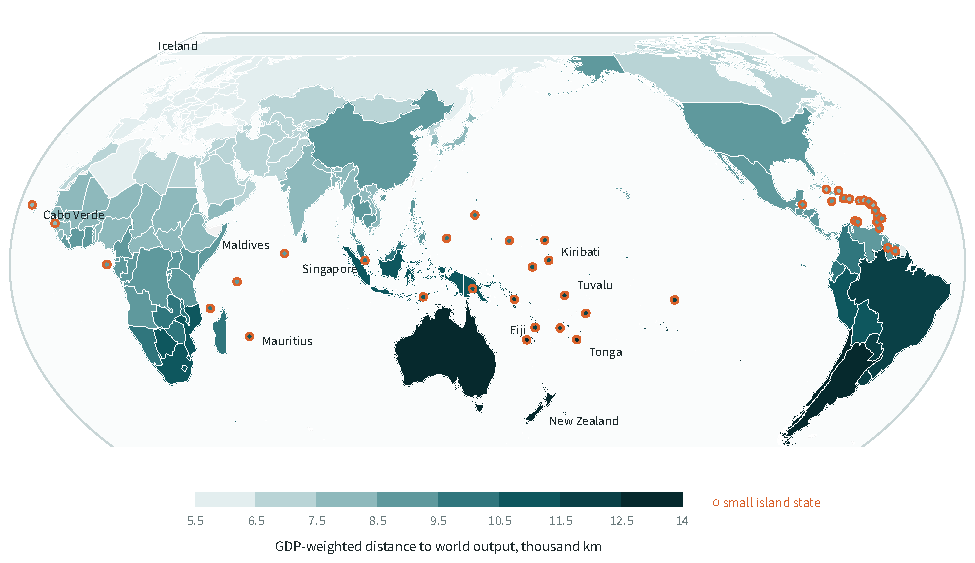
\includegraphics[width=\linewidth]{../figures/remoteness_map.pdf}
  \caption{\takeaway{The Pacific is the far edge of the world economy.}
    Economic remoteness: the GDP-weighted average distance from each economy to
    the rest of world output, \windowStart--\windowEnd. Small island states are
    shown as dots.
    \source{CEPII GeoDist \parencite{mayer2011}; World Bank WDI; UN M49 SIDS list.
    Map: Natural Earth.}}
  \label{fig:map}
\end{figure}


The first finding is that the two dimensions really are distinct. Across
countries the correlation between log remoteness and log population is just
\corrRemotePop. \Cref{fig:map} shows why. The far edge of the world economy is
the South Pacific, together with Australia, New Zealand and the Southern Cone
of Latin America. Several of the archetypal \enquote{peripheral} success stories
are not remote at all on this measure: Iceland (\remoteIcelandKm{} km) and
the Faroe Islands (\remoteFaroesKm{} km) sit between Europe and North America
and are among the \emph{least} remote places on Earth. They are small, not
far. Singapore (\remoteSingaporeKm{} km) and Mauritius (\remoteMauritiusKm{}
km) are moderately remote. This matters for \cref{sec:escape}.

\paragraph{Far versus small.} Which handicap costs more? \Cref{tab:regression}
regresses log income per head (PPP) on log remoteness and log population. On
its own, remoteness has a large negative association with income. Adding
government effectiveness, a crude proxy for institutions, roughly halves the
remoteness coefficient but leaves it large and precisely estimated: holding
governance constant, doubling remoteness is associated with
\regDoubleRemotePctAbs\% lower income per head. Population, by contrast, has a
small coefficient (\regPopTwo{} in column 2); being tiny is not, by itself,
associated with being poor---echoing \textcite{easterly2000}. Being landlocked
carries an extra penalty of about \regLLDCpct\%, consistent with
\textcite{limao2001}. Once distance and governance are accounted for, being a
small island adds nothing significant (\regSIDS, s.e.\ \regSIDSse).

\begin{table}[t]
\centering
\caption{\takeaway{Distance, not size, carries the income penalty.} OLS of log$_{10}$
  GDP per capita (PPP, \windowStart--\windowEnd) on log$_{10}$ remoteness and
  log$_{10}$ population. Robust (HC1) standard errors in parentheses;
  $^{*}p<0.1$, $^{**}p<0.05$, $^{***}p<0.01$.}
\label{tab:regression}
\small\sffamily
% generated by scripts/export_stats.py
\begin{tabular}{@{}lccc@{}}
\toprule
 & (1) & (2) & (3) \\
\midrule
log remoteness & $-2.25^{***}$ & $-1.11^{***}$ & $-1.05^{***}$ \\
 & $(0.35)$ & $(0.18)$ & $(0.21)$ \\[2pt]
log population & $-0.11^{***}$ & $-0.04^{**}$ & $-0.05^{**}$ \\
 & $(0.03)$ & $(0.02)$ & $(0.02)$ \\[2pt]
Government effectiveness &  & $0.41^{***}$ & $0.38^{***}$ \\
 &  & $(0.02)$ & $(0.02)$ \\[2pt]
SIDS &  &  & $-0.07$ \\
 &  &  & $(0.07)$ \\[2pt]
Landlocked (LLDC) &  &  & $-0.19^{***}$ \\
 &  &  & $(0.06)$ \\[2pt]
Constant & $13.71^{***}$ & $8.74^{***}$ & $8.65^{***}$ \\
 & $(1.42)$ & $(0.75)$ & $(0.79)$ \\[2pt]
\midrule
Countries & 197 & 193 & 193 \\
$R^2$ & 0.22 & 0.73 & 0.74 \\
\bottomrule
\end{tabular}

\source{World Bank WDI and WGI; CEPII; author's calculations.}
\end{table}

These are associations, not causal estimates. Governance is itself partly an
outcome of geography and history, so controlling for it may absorb some of
remoteness's true effect, while omitted factors---colonial history above
all \parencite{acemoglu2001}, but also natural resources and language---may
inflate it. The point of \cref{tab:regression} is narrower: in the cross-section,
the burden of the edge loads on \emph{distance}, and the remedies for distance
(connectivity, redundancy, pooled logistics) differ from the remedies for
smallness (pooled institutions, shared services).

\section{From Fixed Cost to Recurring Tax}
\label{sec:tax}

Classic economic geography explains why distance matters even when transport
is cheap. In \citeauthor{krugman1991}'s \parencite*{krugman1991} model, firms
cluster near large markets to exploit economies of scale, and once a core
forms it attracts more activity: the periphery is not just far away but
\emph{left behind} by a self-reinforcing process. \textcite{limao2001} show
how much geography and infrastructure matter: poor infrastructure and
landlocked status can multiply transport costs, and trade volumes fall
steeply as costs rise. \textcite{briguglio1995} catalogued the specific
vulnerabilities of small islands: high per-unit costs of infrastructure and
administration, dependence on a narrow range of exports, exposure to shocks
they cannot influence. And the expected \enquote{death of distance} has been
slow to show up in the data: the estimated effect of distance on trade has
not declined \parencite{disdier2008}, even as transport technology improved
\parencite{hummels2007}.

What changes in an integrated, accelerating world is the \emph{frequency}
with which these costs are paid. A remote economy in 1960 paid a high freight
rate on a few bulk exports and imports. A remote economy in 2025 pays for
every parcel, every software subscription, every cross-border payment, every
specialist consultation and every round of trade or climate negotiations.
The cost is no longer an entry fee; it is a subscription.

\begin{keyidea}[The recurring tax]
Remoteness becomes a \emph{recurring tax on participation} when economic life
consists of many small, frequent, time-sensitive transactions rather than a
few large ones. The tax is levied in freight and insurance, in bandwidth and
latency, in the scarcity of specialists, and in the cost of being present
where rules are made.
\end{keyidea}

\Cref{fig:engine} sketches why the taxes \emph{compound}. Higher trade costs
raise the cost of inputs and shrink the market, weakening the return on
digital investment. Thin and fragile connectivity makes it easier for
skilled people to work for distant employers---or to leave. Their departure
thins the institutions that should negotiate better freight contracts,
spectrum deals, fishing licences and climate finance. Each link is modest; the
loop is what turns geography into a structural gap.

% The "compounding engine": four recurring taxes that feed one another.
\begin{figure}[t]
\centering
\begin{tikzpicture}[
    node distance=1.2cm and 1.6cm,
    tax/.style={rectangle, rounded corners=3pt, draw=teal, line width=0.9pt,
      fill=mist, align=center, font=\sffamily\small, text width=3.3cm,
      minimum height=1.25cm, inner sep=5pt},
    hub/.style={circle, fill=ember, text=white, align=center,
      font=\sffamily\bfseries\footnotesize, minimum size=2.35cm, inner sep=1pt},
    loop/.style={-{Stealth[length=3mm]}, line width=1.2pt, teal, bend left=18},
    lab/.style={font=\sffamily\scriptsize\itshape, text=slate, align=center, fill=white,
      inner sep=1.5pt},
  ]
  \node[hub] (core) {Small, far\\ \& thinly\\ connected};
  \node[tax, above=1.05cm of core] (trade) {\textbf{Trade tax}\\ fewer ships, higher freight, thinner markets};
  \node[tax, right=1.25cm of core] (tech) {\textbf{Connectivity tax}\\ one cable, costly bandwidth, slow repair};
  \node[tax, below=1.05cm of core] (people) {\textbf{Talent tax}\\ skilled emigration, thin specialist cover};
  \node[tax, left=1.25cm of core] (inst) {\textbf{Institutional tax}\\ small bureaucracies, weak bargaining power};

  \draw[loop] (trade.east) to node[lab, above right=-2pt] {costlier inputs,\\ weaker returns to\\ digital investment} (tech.north);
  \draw[loop] (tech.south) to node[lab, below right=-2pt] {remote work pulls\\ talent toward\\ the centre} (people.east);
  \draw[loop] (people.west) to node[lab, below left=-2pt] {fewer specialists\\ to run the state} (inst.south);
  \draw[loop] (inst.north) to node[lab, above left=-2pt] {weaker leverage in\\ trade and finance\\ negotiations} (trade.west);

  \foreach \n in {trade,tech,people,inst}
    \draw[-{Stealth[length=2mm]}, ember, line width=0.7pt, dashed] (core) -- (\n);
\end{tikzpicture}
\caption{\takeaway{The taxes compound.} Each recurring cost of remoteness
  raises the others: the loop, not any single link, is what turns a
  geographic fact into a structural gap. Dashed arrows: smallness and distance
  feed every channel directly.
  \source{Author's schematic, drawing on \textcite{krugman1991,limao2001,briguglio1995}.}}
\label{fig:engine}
\end{figure}


The loop is a hypothesis, not a finding, and the sections that follow test
each link with data. Two things should be held in mind. First, every arrow can
run in reverse: remittances flow back, diasporas carry knowledge home, and
remote places can earn rents from their position (\cref{sec:counter}).
Second, the loop does not say remote places get poorer in absolute terms. It
says their position becomes harder to improve, more volatile and less within
their own control.

\section{Trade: The Distance Tariff}
\label{sec:trade}

Containerisation is the archetypal equaliser: it slashed the cost of moving
goods between big ports. But the container economy rewards scale. Shipping
lines deploy their largest vessels on the busiest routes and serve small
markets with fewer, smaller and less frequent calls, often through
transhipment. For an island importing most of its food, fuel and building
materials, that means higher freight rates, longer and less predictable
lead times, and larger inventories---a tariff levied by geography rather than
by any government.

UNCTAD's Liner Shipping Connectivity Index (LSCI) measures how well a
country is plugged into the global liner network, combining the number of
scheduled calls, the capacity deployed, the number of services and companies,
the size of the largest ships and the number of direct connections \parencite{unctad2026lsci}.
\Cref{fig:lsci} tracks it from \lsciFirstYear{} to \lsciLastYear.

\begin{figure}[t]
\centering
\begin{tikzpicture}
\begin{axis}[edge, height=0.55\linewidth,
    ymode=log, ymin=10, ymax=800,
    ytick={10,20,50,100,200,500}, yticklabels={10,20,50,100,200,500},
    xmin=2006, xmax=2025, xtick={2006,2010,2015,2020,2025},
    x tick label style={/pgf/number format/1000 sep={}},
    ylabel={Liner Shipping Connectivity Index (log scale)},
    legend pos=north east, legend columns=1]
  \addplot[bandTeal, forget plot, name path=hi] table[x=year,y=sids_p75] {\datadir/lsci_groups.csv};
  \addplot[bandTeal, forget plot, name path=lo] table[x=year,y=sids_p25] {\datadir/lsci_groups.csv};
  \addplot[teal, fill opacity=0.12, fill=teal, draw=none, forget plot] fill between[of=hi and lo];
  \addplot[lineEmber] table[x=year,y=hubs] {\datadir/lsci_groups.csv};
  \addlegendentry{2006's ten best-connected hubs (median)}
  \addplot[lineSlate] table[x=year,y=all] {\datadir/lsci_groups.csv};
  \addlegendentry{All countries (median)}
  \addplot[lineTeal] table[x=year,y=sids] {\datadir/lsci_groups.csv};
  \addlegendentry{Small island states (median, band = middle half)}
\end{axis}
\end{tikzpicture}
\caption{\takeaway{Shipping connectivity at the edge has flat-lined.}
  The median small island state scored \sidsMedianLSCIfirst{} in
  \lsciFirstYear{} and \sidsMedianLSCI{} in \lsciLastYear{}, while the median
  country rose by \allLSCIGrowthPct\%. The old hubs lost ground to new ones, so the
  hub-to-island ratio narrowed from \hubSidsRatioFirst{} to \hubSidsRatio{} times.
  Annual averages of quarterly data; index average across countries in Q1 2023 = 100.
  \source{UNCTAD Liner Shipping Connectivity Index; UN M49 SIDS list.}}
\label{fig:lsci}
\end{figure}


The data tell a more nuanced story than the thesis predicts. The headline is
\emph{stagnation at the edge}: the median small island state scored
\sidsMedianLSCIfirst{} in \lsciFirstYear{} and \sidsMedianLSCI{} in
\lsciLastYear{}, essentially unchanged across two decades in which the
median country's connectivity grew by \allLSCIGrowthPct\% and global container
trade expanded. Relative to the median country, island states fell
slightly further behind: the ratio went from \allSidsRatioFirst{} to
\allSidsRatio. Of \nSIDSlsci{} island states with data at both ends,
\nSIDSlsciFell{} saw their index fall. Tuvalu scores \lsciTuvalu; Tonga
\lsciTonga, ranking \lsciTongaRank{} of \nLsci{} economies.

But the gap with the very top did \emph{not} widen. The ten hubs that were
best connected in \lsciFirstYear{} (\hubList) saw their median index fall
from \hubMedianLSCIfirst{} to \hubMedianLSCI{}, as connectivity shifted
towards China and other emerging hubs. The hub-to-island ratio therefore
narrowed, from \hubSidsRatioFirst{} to \hubSidsRatio{} times. A claim that
islands are being left ever further behind the shipping superpowers is not
supported; the more defensible claim is that the global network grew denser
almost everywhere \emph{except} at its smallest, most remote nodes.

\begin{counterpoint}[Islands can climb]
Mauritius raised its LSCI from \lsciMauritiusFirst{} to \lsciMauritius{} over
the period, partly by developing Port Louis as a transhipment centre, and
Singapore built connectivity ranked \lsciSingaporeRank{} of \nLsci{} on a small island
(\cref{sec:escape}). Shipping connectivity is shaped by port investment and
policy, not just by geography.
\end{counterpoint}

The distance tariff also shows up in what islands can export. Goods that are
heavy, perishable or time-sensitive are penalised most, steering remote
economies towards tourism, fish, remittances and rents---activities that
travel by aeroplane, satellite or bank transfer rather than by box. That is
an adaptation, not a failure, but it concentrates risk: when a pandemic grounds
flights or a cyclone closes the port, there are few alternatives.

\section{Technology: Connected but Dependent}
\label{sec:tech}

Almost all international data travel through submarine fibre-optic cables.
For a large coastal country the cable network is a mesh: dozens of
independent systems landing at many points, so a single fault is an
inconvenience. For a small island it is often a single thread. Tonga's
\tongaOutageDays{} days offline in 2022 were not caused by poor management
but by the arithmetic of redundancy.

\begin{figure}[t]
\centering
\begin{tikzpicture}
\begin{axis}[edge, height=0.6\linewidth,
    xmode=log, xlabel={Population, millions (log scale)},
    xmin=0.005, xmax=2000,
    xtick={0.01,0.1,1,10,100,1000}, xticklabels={0.01,0.1,1,10,100,1000},
    ymode=log, ymin=0.8, ymax=80,
    ytick={1,2,3,6,11,21,51}, yticklabels={0,1,2,5,10,20,50},
    ylabel={International submarine cables in service},
    legend pos=north west]
  \addplot[dotsBase, only if={other}{1}] table[x=pop_m,y=cables_p1] {\datadir/plot_countries.csv};
  \addlegendentry{Other coastal economies}
  \addplot[dotsSIDS, only if={sids}{1}] table[x=pop_m,y=cables_p1] {\datadir/plot_countries.csv};
  \addlegendentry{Small island states}
  \addplot[labelled=lab_cables] table[x=pop_m,y=cables_p1] {\datadir/plot_countries.csv};
\end{axis}
\end{tikzpicture}
\caption{\takeaway{Redundancy scales with size, not distance.} Cable counts
  rise with population (correlation of logs \corrCablesPop) but barely vary with
  remoteness (\corrCablesRemote). \nSIDSOneCable{} of \nSIDScables{} small
  island states, including \nPacificOneCable{} in the Pacific, have one
  international cable or none: a single cut takes them offline.
  \source{TeleGeography Submarine Cable Map (cables in service by 2025, excluding
  domestic systems); World Bank WDI.}}
\label{fig:cables}
\end{figure}


\Cref{fig:cables} counts international cables in service in each coastal
economy, using TeleGeography's public map data \parencite{telegeography2026}.
The striking pattern is that redundancy tracks \emph{size}: cable counts rise
steeply with population (correlation \corrCablesPop) and are only weakly
related to remoteness (\corrCablesRemote). Singapore has \cablesSingapore{}
international cables; the median island state \cablesSIDSMedian{}; the median
other coastal economy \cablesOtherMedian. \nSIDSOneCable{} of the
\nSIDScables{} small island states have at most one international cable. Cables
are lumpy, fixed-cost investments; small markets struggle to justify the
second one, which is precisely the one that matters when the first is cut.

Tonga now illustrates the remedy as well as the problem. In May 2026 a branch
of the trans-Pacific Hawaiki cable began service to Vava\okina u, financed with
Australian and New Zealand support, giving the kingdom a second international
link \parencite{aiffp2026tonga}.\footnote{TeleGeography records the branch
under the Hawaiki trunk's \enquote{ready for service} year, 2018; the Tongan
branch itself entered service in 2026. Tonga's count of \cablesTonga{} in
\cref{fig:cables} therefore reflects the 2026 position.}

\paragraph{Connected but dependent.} Connectivity has also changed what
dependence means. A small country's payments, government records, health
systems and schools increasingly run on services hosted abroad, priced in
foreign currency and governed by foreign law. That is mostly a gain---a tiny
administration can rent world-class software---but it means the recurring tax
now includes licence fees, bandwidth charges and the risk that a cut, a
sanction or a platform's change of terms switches services off.

\begin{counterpoint}[Leapfrogging]
Satellite constellations and mobile money cut directly against the thesis.
Low-Earth-orbit satellite internet reaches places where cables never will,
and mobile money has transformed financial access where banks were scarce:
in Kenya it lifted households' ability to share risk
\parencite{jack2014} and reduced poverty \parencite{suri2016}. Fast internet
measurably raised employment where it arrived in Africa
\parencite{hjort2019}.

The test is whether technology helps the edge \emph{faster than the centre}.
On access, it clearly does (\cref{fig:internet}). In 2000 the median
high-income country had \netRatioFirst{} times the share of people online of the
median island state; by \windowEnd{} the ratio was \netRatioLast. The
absolute gap peaked at \netGapPeak{} percentage points in \netGapPeakYear{} and
has since halved to \netGapLast. On \emph{intensity}, convergence is far
slower: fixed broadband lines per 100 people still differ by \bbGapLast{}
(\bbSidsLast{} against \bbHicLast), and in the Pacific the median is
\bbPacificLast. Leapfrogging is real for arrival; the gap persists in depth
of use, price and resilience. Satellite links also add a new dependency, on a
handful of foreign operators.
\end{counterpoint}

\begin{figure}[t]
\centering
\begin{tikzpicture}
\begin{axis}[edge, height=0.52\linewidth,
    xmin=1998, xmax=2023, xtick={2000,2005,2010,2015,2020},
    x tick label style={/pgf/number format/1000 sep={}},
    ymin=0, ymax=100, ylabel={Per 100 people},
    legend style={at={(0.02,0.98)},anchor=north west}]
  \addplot[lineSlate, mark=none] table[x=year,y=net_hic] {\datadir/internet_groups.csv};
  \addlegendentry{Internet users, high income}
  \addplot[lineTeal] table[x=year,y=net_sids] {\datadir/internet_groups.csv};
  \addlegendentry{Internet users, small island states}
  \addplot[lineSlate, dashed, dash pattern=on 4pt off 2pt, line width=1.1pt] table[x=year,y=bb_hic] {\datadir/internet_groups.csv};
  \addlegendentry{Fixed broadband, high income}
  \addplot[lineEmber] table[x=year,y=bb_sids] {\datadir/internet_groups.csv};
  \addlegendentry{Fixed broadband, small island states}
\end{axis}
\end{tikzpicture}
\caption{\takeaway{Access has converged; intensity has not.} In 2000 the
  median rich country had \netRatioFirst{} times the island share of people
  online; by \windowEnd{} it was \netHicLast\% against \netSidsLast\%. Fixed broadband, a proxy for heavy, reliable use, still trails
  by \bbGapLast{} lines per 100 people.
  Medians across countries reporting each year.
  \source{World Bank WDI (ITU data); UN M49 SIDS list.}}
\label{fig:internet}
\end{figure}


\section{Health: Care at a Distance}
\label{sec:health}

Health care is where the recurring tax becomes personal. A small, remote
health system pays it in four currencies: \emph{access} (specialist care,
advanced diagnostics and complex surgery often mean an overseas referral);
\emph{supply} (medicines, vaccines and equipment arrive in small, expensive,
infrequent consignments); \emph{diet} (imported, processed food displaces
local produce); and \emph{workforce} (doctors and nurses are scarce and
mobile).

\paragraph{Workforce.} \Cref{fig:doctors} plots physicians per 1,000 people
against remoteness. The median small island state has \docSIDSMedian{}
doctors per 1,000 and the median Pacific state \docPacificMedian, against
\docHICMedian{} in high-income economies. Remoteness and medical density are
correlated (\corrDocRemote), and the association survives a control for
income: comparing countries with similar income per head, a tenfold increase
in remoteness goes with \docRemoteCoef{} fewer physicians per 1,000 (standard
error \docRemoteSE). In a population of a hundred thousand, the absence of a
single specialist can mean an entire field of medicine is practised only by
referral abroad.

\begin{figure}[t]
\centering
\begin{tikzpicture}
\begin{axis}[edge, height=0.58\linewidth,
    xlabel={Economic remoteness, thousand km}, xmin=5.5, xmax=14.5,
    ymode=log, ymin=0.02, ymax=10, ytick={0.02,0.05,0.1,0.2,0.5,1,2,5,10},
    yticklabels={0.02,0.05,0.1,0.2,0.5,1,2,5,10},
    ylabel={Physicians per 1,000 people (log scale)},
    legend pos=south west]
  \addplot[dotsBase, only if={sids}{0}] table[x=remote_kkm,y=doctors] {\datadir/plot_countries.csv};
  \addlegendentry{Other economies}
  \addplot[dotsSIDS, only if={sids}{1}] table[x=remote_kkm,y=doctors] {\datadir/plot_countries.csv};
  \addlegendentry{Small island states}
  \addplot[labelled=lab_doc] table[x=remote_kkm,y=doctors] {\datadir/plot_countries.csv};
\end{axis}
\end{tikzpicture}
\caption{\takeaway{The further from the centre, the thinner the medical
  workforce.} Median physicians per 1,000: \docSIDSMedian{} in small island
  states, \docPacificMedian{} in the Pacific, \docHICMedian{} in high-income
  economies. Holding income constant, a tenfold rise in remoteness is associated with
  \docRemoteCoef{} fewer doctors per 1,000 (s.e.\ \docRemoteSE). Latest year 2013--23.
  \source{World Bank WDI (WHO data); CEPII; author's remoteness index.}}
\label{fig:doctors}
\end{figure}


\paragraph{Diet and disease.} The Pacific has some of the world's highest
rates of diabetes. In NCD-RisC's estimates \parencite{ncdrisc2024}, the
highest age-standardised prevalence in 2022 was in \diabTopName{}
(\diabTopValue\%), and \diabTopTenPacific{} of the ten highest-prevalence
countries are Pacific island states (\cref{fig:diabetes}). Imported, cheap,
energy-dense foods---refined flour, sugar, fatty meat cuts---have displaced
traditional diets, and Pacific governments have experimented with trade and
tax measures to push back \parencite{snowdon2013}.

\begin{figure}[t]
\centering
\begin{tikzpicture}
\begin{axis}[edge, height=0.52\linewidth,
    xmin=1990, xmax=2022, xtick={1990,2000,2010,2022},
    x tick label style={/pgf/number format/1000 sep={}},
    ymin=0, ymax=36, ylabel={Adults with diabetes, \% (age-standardised)},
    legend style={at={(0.02,0.98)},anchor=north west}]
  \addplot[lineEmber] table[x=year,y=pacific] {\datadir/diabetes_groups.csv};
  \addlegendentry{Pacific island states (median)}
  \addplot[lineTeal] table[x=year,y=sids] {\datadir/diabetes_groups.csv};
  \addlegendentry{All small island states (median)}
  \addplot[lineSlate] table[x=year,y=all] {\datadir/diabetes_groups.csv};
  \addlegendentry{All countries (median)}
\end{axis}
\end{tikzpicture}
\caption{\takeaway{Island diabetes rates were high and kept rising.}
  The median Pacific state went from \diabPacificNinety\% to \diabPacificNow\%
  between 1990 and 2022; the median country from \diabAllNinety\% to
  \diabAllNow\%. The rest of the world is catching up, so the relative gap
  narrowed (from \diabPacificRatioNinety{} to \diabPacificRatioNow{} times) even
  as the absolute gap held. Mean of male and female estimates, adults 18+.
  \source{NCD-RisC \parencite{ncdrisc2024}; UN M49.}}
\label{fig:diabetes}
\end{figure}


Two cautions apply. First, diet change has many causes: urbanisation,
incomes, physical activity, genetics, marketing and culture all play a part,
and the data here cannot apportion blame to remoteness or trade. The claim
is only that remote, import-dependent food systems make healthy diets
\emph{more expensive} and treatment harder to deliver---a tax on the cure as
well as a contributor to the disease. Second, the relative gap is narrowing,
for an unhappy reason: the rest of the world is catching up. The Pacific
median was \diabPacificRatioNinety{} times the global median in 1990 and
\diabPacificRatioNow{} times in 2022. What remote systems lack is not
awareness of the problem but the scale to manage it: dialysis units, retinal
screening, endocrinologists and reliable insulin supply chains.

\section{People: The Quiet Exodus}
\label{sec:people}

The most valuable export of many small places is people. For an individual
nurse in Suva or engineer in Kingston, emigration is often a rational and
welcome choice, and the evidence that skilled emigrants themselves gain a
great deal is strong \parencite{gibson2012}. For the country, the arithmetic
is harder. A small population can afford to lose few specialists, and the
ones most likely to leave are the most educated
\parencite{docquier2012,gibson2011}.

\begin{figure}[t]
\centering
\begin{tikzpicture}
\begin{axis}[edge, height=0.6\linewidth,
    xmode=log, xlabel={Population, millions (log scale)},
    xmin=0.005, xmax=2000,
    xtick={0.01,0.1,1,10,100,1000}, xticklabels={0.01,0.1,1,10,100,1000},
    ymin=0, ymax=100,
    ylabel={Tertiary-educated emigration rate, 2010 (\%)},
    legend pos=north east]
  \addplot[dotsBase, only if={sids}{0}] table[x=pop_m,y=emig_high_2010] {\datadir/plot_countries.csv};
  \addlegendentry{Other economies}
  \addplot[dotsSIDS, only if={sids}{1}] table[x=pop_m,y=emig_high_2010] {\datadir/plot_countries.csv};
  \addlegendentry{Small island states}
  \addplot[labelled=lab_emig] table[x=pop_m,y=emig_high_2010] {\datadir/plot_countries.csv};
\end{axis}
\end{tikzpicture}
\caption{\takeaway{Small places lose their graduates.} Share of each country's
  university-educated adults living in 20 OECD destinations. The median small island
  state lost \emigSIDSMedian\%; countries with more than 20 million people lost
  \emigLargeMedian\%. Of the \nEmigOverHalf{} countries losing more than half their
  graduates, \nEmigOverHalfSIDS{} are small island states. Population
  \windowStart--\windowEnd; emigration 2010, the latest year available.
  \source{IAB brain-drain data \parencite{brucker2013}; World Bank WDI.}}
\label{fig:emigration}
\end{figure}


\Cref{fig:emigration} uses the IAB brain-drain dataset
\parencite{brucker2013}, which reports the share of each country's
university-educated adults living in 20 OECD destinations. The pattern is
stark. The median small island state had lost \emigSIDSMedian\% of its
graduates by 2010; the median country \emigAllMedian\%; countries with more
than 20 million people \emigLargeMedian\%. Across countries, the
tertiary emigration rate is strongly negatively correlated with log population
(correlation \corrEmigPop). Of the \nEmigOverHalf{} countries that had lost more than
half their graduates, \nEmigOverHalfSIDS{} are small island states. Emigration
is also highly selective: in the median island state the graduate emigration
rate is \emigSelectivity{} times the overall rate. Tonga's graduate emigration
rate was \emigTonga\%.

\paragraph{The money comes back.} The exodus is not a one-way loss. Diasporas
send money home, and for many small states remittances are a pillar of the
economy (\cref{fig:remittances}). \remitTopName{} is the most
remittance-dependent economy in the world, at \remitTopValue\% of GDP;
Samoa receives \remitSamoa\%. The median island state receives
\remitSIDSMedian\% of GDP, against \remitWorldMedian\% for the median
economy. Remittances smooth consumption and pay school fees; they also tie
household welfare to labour markets in Auckland, Sydney and Los Angeles, and
to the cable and banking links that carry the transfers---the links that
failed in Tonga in 2022.

\begin{figure}[t]
\centering
\begin{tikzpicture}
\begin{axis}[edge, height=0.62\linewidth, width=0.86\linewidth,
    xbar, bar width=6pt, bar shift=0pt, xmin=0, xmax=45,
    xlabel={Personal remittances received, \% of GDP (\windowStart--\windowEnd{} average)},
    ytick={0,...,19}, yticklabels from table={\datadir/remittances_top.csv}{short},
    y tick label style={font=\sffamily\scriptsize,color=ink},
    ymin=-0.7, ymax=19.7, enlarge y limits=false,
    grid=none, xmajorgrids=true, axis lines*=left, y axis line style={draw=none},
    ytick style={draw=none},
    nodes near coords, nodes near coords style={font=\sffamily\tiny,color=slate},
    every node near coord/.append style={/pgf/number format/.cd,fixed,precision=0},
    legend style={at={(0.98,0.04)},anchor=south east}]
  \addplot[fill=ember, draw=none, only if={sids}{1}] table[x=remittances_gdp,y=pos] {\datadir/remittances_top.csv};
  \addlegendentry{Small island state}
  \addplot[fill=teal, draw=none, only if={lldc}{1}] table[x=remittances_gdp,y=pos] {\datadir/remittances_top.csv};
  \addlegendentry{Landlocked developing}
  \addplot[fill=haze, draw=none, only if={other}{1}] table[x=remittances_gdp,y=pos] {\datadir/remittances_top.csv};
  \addlegendentry{Other}
\end{axis}
\end{tikzpicture}
\caption{\takeaway{The diaspora is part of the economy.}
  The \remitTopN{} economies most dependent on remittances. \remitTopName{}
  tops the world at \remitTopValue\% of GDP; \nRemitTopSIDS{} of the
  \remitTopN{} are small island states and \nRemitTopLLDC{} are landlocked.
  \source{World Bank WDI.}}
\label{fig:remittances}
\end{figure}


The policy question is not how to stop people leaving---that would be
neither possible nor right---but how to make migration \emph{circular}, so
that skills, savings and networks return. \Cref{sec:paying} takes this up.

\section{Climate: Exposure Without Influence}
\label{sec:climate}

Globalisation did not cause cyclones or sea-level rise, and this paper does
not claim it did. The connection is an \emph{asymmetry}: the places most
exposed to climate hazards contribute least to emissions and have the least
say over global responses. Remoteness and smallness sharpen that asymmetry.
A single cyclone can damage a large share of a small island's housing stock and
infrastructure at once, and recovery depends on imported materials, foreign
contractors and international finance---all subject to the distance tariff.

\begin{figure}[t]
\centering
\begin{tikzpicture}
\begin{axis}[edge, height=0.6\linewidth,
    xmode=log, xmin=0.03, xmax=60,
    xtick={0.1,0.3,1,3,10,30}, xticklabels={0.1,0.3,1,3,10,30},
    xlabel={CO$_2$ emissions per person, tonnes (log scale)},
    ymode=log, ymin=0.005, ymax=100,
    ytick={0.01,0.1,1,10,100}, yticklabels={0.01,0.1,1,10,100},
    ylabel={Disaster displacements per 1,000 people, yearly (log)},
    legend pos=south east]
  \addplot[dotsBase, only if={sids}{0}] table[x=co2pc,y=displaced_per_k] {\datadir/plot_countries.csv};
  \addlegendentry{Other economies}
  \addplot[dotsSIDS, only if={sids}{1}] table[x=co2pc,y=displaced_per_k] {\datadir/plot_countries.csv};
  \addlegendentry{Small island states}
  \addplot[labelled=lab_climate] table[x=co2pc,y=displaced_per_k] {\datadir/plot_countries.csv};
\end{axis}
\end{tikzpicture}
\caption{\takeaway{Exposure without influence.} Small island states account
  for \sidsCOshare\% of the world's CO$_2$ emissions (and \sidsPopShare\% of its
  people) yet the median island state sees \dispSIDSRatio{} times as many
  disaster displacements per head as the median other country. \nDispTopTenSIDS{} of the ten most-displaced
  economies are islands. Emissions \windowStart--\windowEnd{} average; displacements
  2008--2023 average (years without a report counted as zero; countries without any report omitted).
  \source{World Bank WDI (EDGAR emissions; IDMC displacement data).}}
\label{fig:climate}
\end{figure}


\Cref{fig:climate} sets per-person carbon emissions against a measure of
realised exposure: new disaster displacements per 1,000 residents, averaged
over 2008--2023 (IDMC data via the World Bank). Small island states account for \sidsCOshare\% of
global CO$_2$ emissions and \sidsPopShare\% of world population; the Pacific
island states for just \pacificCOshare\%. Median emissions are
\coPacificMedian{} tonnes a head in the Pacific and \coSIDSMedian{} in all
island states, against \coHICMedian{} in high-income economies. Yet the
median island state records \dispSIDSRatio{} times as many disaster
displacements per head as the median other economy, and \nDispTopTenSIDS{}
of the ten most-affected countries are islands; \dispTopName{} tops the list
with \dispTopValue{} displacements per 1,000 people a year. Low-lying atolls
face the slow-onset threat too: \lowElevMarshall\% of Marshall Islanders and
\lowElevTuvalu\% of Tuvaluans live less than five metres above sea level.

Exposure alone is not destiny either: \lowElevNetherlands\% of the Dutch also
live below five metres, and the Netherlands is rich and safe because it can
afford to engineer its coast. The asymmetry that matters is between exposure
and the \emph{capacity} to adapt---money, engineers, insurance and
negotiating weight---and capacity is exactly what the recurring tax erodes.

\section{Acceleration: Why a Small Lag Grows}
\label{sec:accel}

If technologies now spread faster, why worry about lags? Because what
matters for income is not whether a technology has \emph{arrived} but how
intensively it is \emph{used}. \textcite{comin2010} showed that adoption lags
have shortened dramatically across successive technologies;
\textcite{comin2018} found that while adoption lags converged, the intensity of use in poor
countries relative to rich ones diverged---and that the productivity trends
implied by these two patterns resemble the actual divergence of world incomes
over the past two centuries.

\begin{figure}[t]
\centering
\begin{tikzpicture}
\begin{axis}[edge, height=0.58\linewidth,
    xmin=0, xmax=72, xlabel={Median adoption lag behind the first five adopters, years},
    ymode=log, ymin=4, ymax=60, ytick={5,10,20,50}, yticklabels={5$\times$,10$\times$,20$\times$,50$\times$},
    ylabel={Intensity gap, richest quarter vs poorest half},
    legend pos=north east]
  \addplot[only marks, mark=*, mark size=2.4pt, mark options={fill=haze,draw=slate}, only if={era}{industrial}]
    table[x=lag,y=gap_ratio] {\datadir/adoption.csv};
  \addlegendentry{Industrial era (frontier before 1915)}
  \addplot[only marks, mark=square*, mark size=2.2pt, mark options={fill=teal,draw=white}, only if={era}{mid}]
    table[x=lag,y=gap_ratio] {\datadir/adoption.csv};
  \addlegendentry{Mid-century (1915--1960)}
  \addplot[only marks, mark=diamond*, mark size=3pt, mark options={fill=ember,draw=white}, only if={era}{digital}]
    table[x=lag,y=gap_ratio] {\datadir/adoption.csv};
  \addlegendentry{Digital (after 1975)}
  \addplot[labelled=label] table[x=lag,y=gap_ratio] {\datadir/adoption.csv};
\end{axis}
\end{tikzpicture}
\caption{\takeaway{Technologies arrive faster but are used less
  equally.} For \nTechs{} technologies, the typical country adopted
  industrial-era inventions decades after the frontier, but digital ones within
  about a decade. Yet in 2000 the richest quarter of countries used computers and
  mobile phones \gapComputer{} and \gapCell{} times as intensively per person
  as the poorest half, against \gapOldMedian{} times for the median
  pre-1950 technology. Digital technologies were young in 2000, which
  inflates their gaps; see text.
  \source{CHAT \parencite{comin2009chat}; author's calculations following
  \textcite{comin2010,comin2018}.}}
\label{fig:adoption}
\end{figure}


\Cref{fig:adoption} reproduces that pattern descriptively with the CHAT
dataset \parencite{comin2009chat}. For each of \nTechs{} technologies, the
horizontal axis shows how long the typical country took to adopt it after the
first five adopters; the vertical axis shows how many times more intensively
the richest quarter of countries used it, per person, than the poorest half.
Lags shrank from \lagRail{} years for passenger railways and
\lagTelephone{} for the telephone to \lagCell{} for mobile phones and
\lagComputer{} for computers. But intensity gaps grew: \gapRail-fold for
railways and \gapTV-fold for television, \gapCell-fold for mobile phones and
\gapComputer-fold for computers in 2000. Across technologies, shorter lags
go with \emph{larger} gaps (correlation \corrLagGap).

An honest caveat: in 2000 mobile phones and computers were young, and gaps
during early diffusion are naturally large; some of the difference will close,
as it has for internet access (\cref{fig:internet}). The structural point
survives the caveat. When the frontier moves fast, a country that adopts
late and uses lightly is chasing a moving target, and each new layer of
technology builds on the last. Being a few years and a few multiples behind
in broadband becomes being further behind in cloud services, in data-driven
logistics, in AI.

\paragraph{Thin layers.} Three further mechanisms turn small lags into
lasting gaps in small, remote places.
\emph{Language}: digital services, voice assistants and now AI models are
built first, and best, for languages with many speakers and much text; a
language with a hundred thousand speakers is served last, if at all.
\emph{Food systems}: once local agriculture and supply chains have been
displaced by imports, the knowledge and infrastructure to rebuild them
decays. \emph{Thin institutions}: a ministry with a handful of staff must
cover the same range of international standards, negotiations and
regulations as one with thousands. Each new technology---data protection,
digital trade rules, AI governance---adds a portfolio but not a person.

\section{Who Escapes?}
\label{sec:escape}

If remoteness were destiny, Iceland, the Faroe Islands, Singapore and
Mauritius would be poor. They are not. Any account of the edge must explain
them, and \cref{tab:escape} lines them up against the median Pacific island
state.

\begin{table}[t]
\centering
\caption{\takeaway{The escapees are small but mostly not far, and all built
  institutions or hubs.} Selected indicators,
  \windowStart--\windowEnd{} averages unless stated; Pacific column is the
  median across Pacific small island states.}
\label{tab:escape}
\small\sffamily
% generated by scripts/export_stats.py
\begin{tabular}{@{}l*{5}{r}@{}}
\toprule
 & Iceland & Faroe Is. & Singapore & Mauritius & \makecell[r]{Pacific\\SIDS} \\
\midrule
Population (thousands) & 373 & 53 & 5{,}680 & 1{,}262 & 128 \\
Remoteness (km) & 5{,}854 & 5{,}750 & 9{,}844 & 10{,}568 & 11{,}565 \\
GDP per capita, PPP (\$) & 65{,}036 & 68{,}941 & 127{,}296 & 24{,}543 & 6{,}018 \\
Government effectiveness & 1.65 & --- & 2.08 & 0.92 & -0.06 \\
Shipping connectivity (2025) & 29 & 21 & 614 & 79 & 26 \\
International cables & 4 & 2 & 32 & 4 & 2 \\
Tertiary emigration, 2010 (\%) & 17 & --- & 10 & 63 & 28 \\
Tourism, \% of exports (2015--19) & --- & --- & 3 & 34 & 38 \\
\bottomrule
\end{tabular}

\source{World Bank WDI and WGI; CEPII; UNCTAD; TeleGeography; IAB. --- = not available.}
\end{table}

Three lessons stand out.

\paragraph{Lesson 1: most escapees are small, not far.} Iceland and the
Faroes are among the \emph{least} remote economies on Earth by GDP-weighted
distance: they sit between the two largest consumer markets in the North
Atlantic. Their populations are tiny (\popIcelandK{} and \popFaroesK{}
thousand), but \cref{sec:edge} found that size alone carries little income
penalty. Their success is a warning against treating all \enquote{peripheries}
alike---and partial evidence \emph{for} the paper's distinction between
distance and scale. The genuinely far edge, the South Pacific, has no
equivalent success story among its small states.

\paragraph{Lesson 2: turn position into rent.} Each escapee found something
the centre needed and could only get from them. Iceland and the Faroes
control rich fisheries and, in Iceland's case, cheap geothermal and hydro
power. Mauritius built export processing, financial services and tourism;
tourism alone earned \tourismMauritius\% of its exports before the pandemic.
Singapore made itself the hub that others must route through---the
opposite of the edge. Its shipping connectivity index is \lsciSingapore{} against a Pacific median
of \pacificMedianLSCI, and it has \cablesSingapore{} international cables.

\paragraph{Lesson 3: institutions do the heavy lifting.} All four score far
above the Pacific median on government effectiveness (Singapore \govSingapore,
Iceland \govIceland, Mauritius \govMauritius, against \govPacificMedian{}),
and in \cref{tab:regression} governance absorbed about half of the raw
remoteness penalty. Good institutions are partly a product of history,
including colonial history \parencite{acemoglu2001}, and cannot simply be
imported; but they are the lever over which small states have most control.

\begin{counterpoint}[Escape is not immunity]
Even escapees pay the talent tax. Mauritius had lost \emigMauritius\% of
its university graduates to the OECD by 2010, far more than Iceland
(\emigIceland\%) or Singapore (\emigSingapore\%), which can offer graduates
careers at home. Iceland's 2008 banking collapse showed how a small economy that
plugs into global finance can be overwhelmed by it. Escape is a trajectory,
not a permanent state.
\end{counterpoint}

\section{Counterarguments}
\label{sec:counter}

The argument has real weaknesses. The strongest objections are set out here
in their own words, with what the evidence in this paper says about each.

\begin{counterpoint}[1\enspace ``Remote places got richer, not poorer'']
True. Absolute living standards have risen across almost all small and remote
states, and nothing here shows otherwise. The claim is relative: about
position, volatility and control. Where the data show relative gaps
narrowing---internet access, shipping relative to the old hubs, diabetes
relative to the world---the paper says so.
\end{counterpoint}

\begin{counterpoint}[2\enspace ``It's governance, not geography'']
Partly. Government effectiveness absorbs about half of the cross-country
income penalty of remoteness in \cref{tab:regression}, and colonial history
and resource endowments are uncontrolled confounders. But distance retains a
large, precisely estimated association with income even after governance is
held fixed---and the direction of causation between geography and governance
plausibly runs both ways, since thin institutions are themselves one of the
taxes of smallness.
\end{counterpoint}

\begin{counterpoint}[3\enspace ``Technology will solve it'']
For access, technology is solving it (\cref{fig:internet}). Satellite internet
and mobile money are genuine equalisers. But redundancy, intensity of use,
price and the capacity to build on each layer are not converging as quickly
(\cref{fig:cables,fig:adoption}), and new technologies create new
dependencies on a small number of foreign providers.
\end{counterpoint}

\begin{counterpoint}[4\enspace ``Small states are not passive victims'']
Correct, and important. Small states earn real rents from their position.
The Parties to the Nauru Agreement, a bloc of Pacific states, transformed their
bargaining power over foreign tuna fleets with the Vessel Day Scheme, which
sells fishing days rather than licences \parencite{aqorau2009}. Several
states run international ship registries. Tuvalu licenses its country-code
domain, .tv, to a global registry operator \parencite{pina2021tv}. These are
evidence of agency---and of the edge being turned into an asset.
\end{counterpoint}

\begin{counterpoint}[5\enspace ``Diet and health have many causes'']
Agreed. The paper does not attribute Pacific diabetes rates to remoteness or
trade. It argues only that remote, import-dependent food systems and thin
health workforces make prevention and treatment more costly.
\end{counterpoint}

\begin{counterpoint}[6\enspace ``Globalisation didn't cause climate change in the Pacific'']
Also agreed. The climate argument is about an asymmetry of exposure versus
influence, not causation by trade.
\end{counterpoint}

\section{Paying Down the Tax}
\label{sec:paying}

If remoteness is a recurring tax, policy can lower the rate. The aim is not to
abolish distance but to stop it compounding. Six levers follow from the
evidence above.

\paragraph{1. Pool scale.} The cheapest way to be less small is to share.
Regional bulk procurement of medicines and fuel, shared shipping contracts,
regional universities and regulators, and joint diplomatic missions spread
fixed costs over larger populations. The Pacific already does some of this;
the evidence on thin institutions (\cref{sec:accel}) argues for much more,
especially in fast-moving areas such as cybersecurity, data protection and AI
regulation, where no small ministry can keep up alone.

\paragraph{2. Buy redundancy.} \nSIDSOneCable{} island states depend on one
cable or none. A second cable, a satellite back-up and pre-positioned repair
arrangements are insurance, and should be financed as insurance: by pooling
risk across many states rather than asking each tiny market to justify a
second system commercially. Tonga's new branch on the Hawaiki cable, built
with Australian and New Zealand support four years after the
\tongaOutageDays-day blackout, shows both what is possible and how long it
can take \parencite{aiffp2026tonga}.

\paragraph{3. Finance vulnerability, not income.} Many small states are
\enquote{too rich} for concessional finance by income per head while being far
more exposed than poorer countries (\cref{fig:climate}). Allocating
concessional finance and climate funds by measured vulnerability, rather than
by income alone, would match money to risk.

\paragraph{4. Bargain as a bloc.} The tuna Vessel Day Scheme shows what
coordinated small states can extract when they control something scarce
\parencite{aqorau2009}. The same logic applies to shipping and data
contracts, to landing rights for cables and satellites, and to climate
negotiations, where island coalitions have long punched above their weight.

\paragraph{5. Make talent circular.} Migration will continue, and it brings
remittances and skills (\cref{sec:people}). Policy can tilt it towards
circulation: portable pensions and qualifications, remote-work arrangements
that let diaspora professionals serve home institutions, bonded scholarships
paired with good jobs at home, and temporary labour schemes with real skill
transfer.

\paragraph{6. Build technology for small languages.} Digital public
infrastructure, open-source tools and AI models trained on small languages
are public goods with near-zero marginal cost. Funding them regionally---and
insisting that platforms serve small-language markets---lowers the newest and
fastest-compounding layer of the tax.

\section{Conclusion: Peripherality as a Trajectory}
\label{sec:conclusion}

The flat-world promise was half right. Falling costs of moving goods, data
and people have brought the edge closer in absolute terms: more islanders are
online, connected and richer than ever. But integration has also turned
remoteness into a recurring tax, paid in freight, bandwidth, talent and
negotiating capacity, and the taxes reinforce one another.

The data in this paper support that picture in some places and complicate it
in others. Distance, more than smallness, carries an income penalty. Shipping
connectivity at the smallest, most remote nodes has stagnated while the
network thickened elsewhere. Redundancy scales with size, and a single cable
still carries entire national economies. Small islands lose most of their
graduates. Technologies now arrive quickly but are used far less intensively.
Against this, internet access has converged dramatically, gaps with the old
shipping hubs have narrowed, and four peripheral economies show that the edge
can be escaped---though the richest of them turn out to be small rather than
far.

The right conclusion is neither fatalism nor complacency. Peripherality is a
trajectory, not a location. Whether a place moves towards the centre or away
from it depends on how it pools scale, buys redundancy, finances its
exposure, bargains with others and keeps its people connected. In an
accelerating world, the cost of standing still at the edge rises every year;
so does the return to acting early.

\begin{pullquote}
The edge is not a place. It is a direction of travel.
\end{pullquote}


\appendix
\section{Data and Methods}
\label{app:data}

\paragraph{Reproducibility.} Every number in the text, tables and figures is
generated by the scripts in the accompanying repository from public sources,
cached on first download with a SHA-256 checksum. Running \texttt{make all}
rebuilds the paper; \texttt{data/SOURCES.md} lists each dataset's URL, access
date and licence.

\paragraph{Country groups.} Small Island Developing States (SIDS) and
Landlocked Developing Countries (LLDC) follow the UN M49 classification
\parencite{unm49}. \enquote{Pacific} denotes SIDS in Melanesia, Micronesia and
Polynesia. Of \nSIDSunList{} SIDS in the M49 list, \nSIDS{} appear in World Bank
data and are used here. Group statistics are unweighted medians across
countries, so that no single large member dominates.

\paragraph{Remoteness.} For country $i$,
\begin{equation}
  R_i \;=\; \sum_{j\neq i} \frac{Y_j}{\sum_{k\neq i} Y_k}\, d_{ij},
\end{equation}
where $Y_j$ is GDP in current US dollars (\windowStart--\windowEnd{}
average, World Bank) and $d_{ij}$ is the great-circle distance between the
most populous cities of $i$ and $j$ from CEPII's GeoDist \parencite{mayer2011}.
GeoDist (2011) uses some superseded country codes; successor states inherit
their predecessor's distances (e.g. Montenegro from Serbia and Montenegro;
South Sudan from Sudan; Curaçao and Sint Maarten from the Netherlands
Antilles). Taiwan has distances but no World Bank GDP, so it carries no
weight. Remoteness is computed for \nCountriesRemote{} economies.

\paragraph{Regression.} \Cref{tab:regression} reports OLS with
heteroskedasticity-robust (HC1) standard errors. All variables are
\windowStart--\windowEnd{} averages; government effectiveness is the
Worldwide Governance Indicators estimate. Coefficients on log$_{10}$ variables
are elasticities; the \enquote{doubling} effect is $2^{\beta}-1$.

\paragraph{Shipping.} UNCTAD's quarterly LSCI is averaged to calendar years
(complete years only). \enquote{Hubs} are the ten highest-scoring economies in
\lsciFirstYear{}, fixed at the start to avoid selecting on later outcomes.

\paragraph{Cables.} From TeleGeography's public map data, a cable counts
for a country if it is in service (not planned, ready-for-service year up to
2025) and lands in at least two countries. Branch systems are recorded by
TeleGeography under their trunk's ready-for-service year.

\paragraph{Technology adoption.} For each CHAT technology, adoption is the
first year with a positive value. The frontier year is the year the fifth
country adopted; the lag is the median across later adopters. The intensity
gap is the ratio of median per-capita use in the richest quarter of
countries (CHAT real GDP per capita) to that in the poorest half, in the last
year up to 2000 in which at least 40 countries report. Technologies whose
records begin simultaneously for many countries (left-censored) are excluded.
This is a descriptive analogue of \textcite{comin2010,comin2018}, not a
replication.

\paragraph{Other variables.} Physicians per 1,000: latest World Bank value
2013--2023. Diabetes: NCD-RisC age-standardised prevalence, adults 18+,
simple mean of male and female estimates. Graduate emigration: IAB, 2010,
population 25+, 20 OECD destinations. Displacement: IDMC new disaster
displacements via the World Bank, 2008--2023, per 1,000 residents, with
unreported years counted as zero. Emissions: CO$_2$ excluding land use, tonnes
per person (EDGAR via the World Bank).

\paragraph{Departures from the original plan.} The ND-GAIN vulnerability
index and ITU broadband prices could not be downloaded automatically when the
pipeline was built (their servers refused scripted access), and the WHO
Global Health Observatory API was unavailable; WorldRiskIndex was considered
but rejected because its exposure component scales with absolute population
and so ranks large countries as most exposed. The climate figure therefore
uses displacement per head, and diabetes uses NCD-RisC. See \texttt{TODO.md}.


\clearpage
\phantomsection
\addcontentsline{toc}{section}{References}
\printbibliography[heading=bibnumbered,title={References}]

\end{document}
